
\documentclass[runningheads]{llncs}
\usepackage[text={150mm,220mm},centering]{geometry}
\usepackage{graphicx}
\usepackage{float}
\usepackage{listings}

\begin{document}
\title{\large{Computational Intelligence Laboratory Exercise 2}}
\author{\large{Student Name: ChangXu \\ % Please write your name here
CCNU Student Number: 2019180034 \\ % Please write your CCNU student number here
UOW Student Number: 6643048}}  % Please write your UOW student number here


\authorrunning{CCNU Wollongong Joint Institute}
\institute{Central China Normal University Wollongong Joint Institute}

\maketitle


%-----------Please write your solutions to the questions in the assignment from here.---------------

\section{Task One}
\begin{figure}[H]
    \centering
    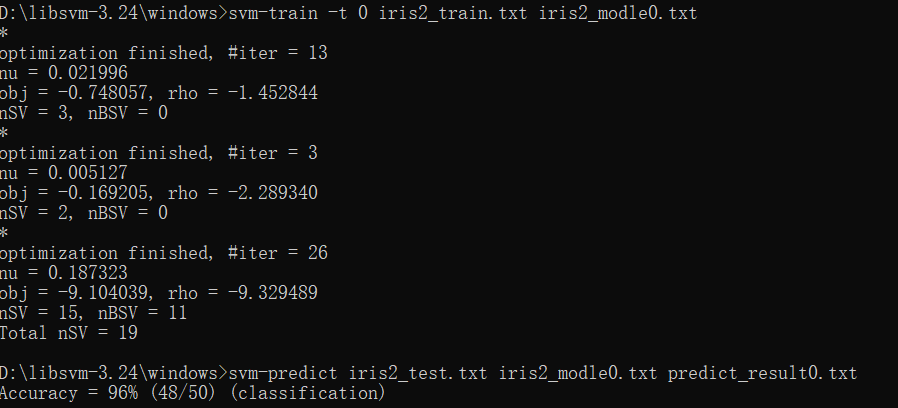
\includegraphics[scale=0.8]{liner2.PNG}  
\end{figure}
\begin{figure}[H]
    \centering
    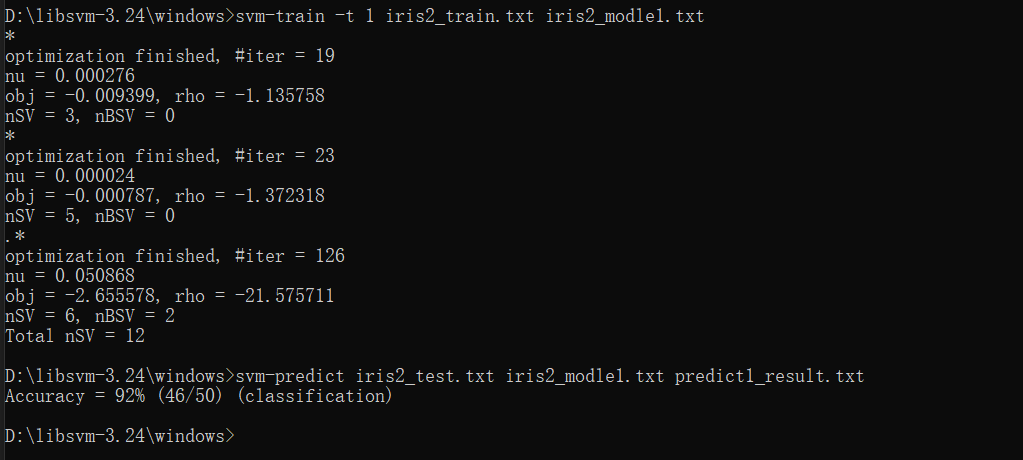
\includegraphics[scale=0.8]{poly2.PNG}  
\end{figure}

\begin{figure}[H]
    \centering
    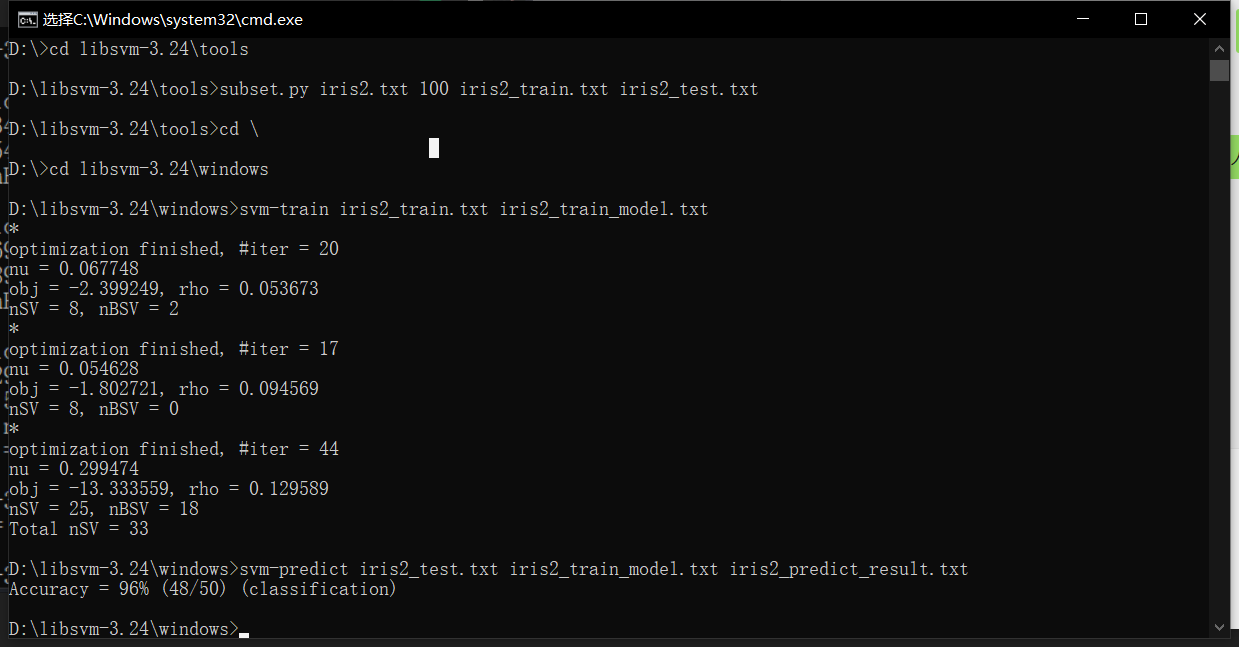
\includegraphics[scale=0.8]{RBF2.PNG}
\end{figure}

Freom the result of predict accurancy, we can know 
that using Polynomial Kernel perform little worse
than the left two Kernel way using libsvm toolsbox in
classifying iris\_data.
\end{document}
